\documentclass{amsart}
\usepackage{amsmath, amssymb}
\usepackage{tikz-cd}
\usepackage{mathbbol} % mathbb on greek letters

% hyperref
\usepackage[bookmarks=true, linktocpage=true,
bookmarksnumbered=true, breaklinks=true,
pdfstartview=FitH, hyperfigures=false,
plainpages=false, naturalnames=true,
colorlinks=true, pagebackref=true,
pdfpagelabels]{hyperref}
\hypersetup{
	colorlinks,
	citecolor=blue,
	filecolor=blue,
	linkcolor=blue,
	urlcolor=blue
}

% layout
\setlength{\textwidth}{\paperwidth}
\addtolength{\textwidth}{-1.85in}
\setlength{\textheight}{\paperheight}
\addtolength{\textheight}{-2in}
\calclayout

% Updating to MSC2020
\makeatletter
\@namedef{subjclassname@2020}{%
	\textup{2020} Mathematics Subject Classification}
\makeatother

% elements
\renewcommand{\P}{\mathcal{P}}
\renewcommand{\S}{\mathbb{S}}
\newcommand{\A}{\mathcal{A}ssoc}
\newcommand{\M}{\mathcal{M}}

% sets
\newcommand{\Z}{\mathbb{Z}}
\newcommand{\id}{\mathrm{id}}
\newcommand{\End}{\mathrm{End}}
\newcommand{\Hom}{\mathrm{Hom}}
\newcommand{\Bij}{\mathfrak{Bij}}
\newcommand{\G}{\mathfrak{G}}

% categories
\newcommand{\Ch}{\mathsf{Mod}_R}
\newcommand{\Alg}{\mathsf{Alg}}
\newcommand{\coAlg}{\mathsf{coAlg}}
\newcommand{\sSet}{\mathsf{sSet}}
\newcommand{\cSet}{\mathsf{cSet}}
\newcommand{\nSet}{\mathsf{nSet}}
\newcommand{\Mon}{\mathsf{Mon}}

% functors
\DeclareMathOperator*{\tensor}{\otimes}
\newcommand{\chains}{N_\bullet}
\newcommand{\cochains}{N_\bullet}
\newcommand{\Uleft}{U_{left}}
\newcommand{\Uright}{U_{right}}
\newcommand{\op}{\mathrm{op}}
\DeclareMathOperator*{\colim}{colim}
\newcommand{\cobar}{\Omega}
\newcommand{\gcobar}{\mathbb{\Omega}}

% environments
\newtheorem{theorem}{Theorem}
\newtheorem{proposition}[theorem]{Proposition}
\theoremstyle{definition}
\newtheorem{definition}[theorem]{Definition}

% comments
\newcommand{\anibal}[1]{\textcolor{blue}{#1}}

% drawings
\usetikzlibrary{arrows,decorations.markings}
\tikzset{myptr/.style={decoration={markings,mark=at position 1 with %
			{\arrow[scale=2,>=stealth]{>}}},postaction={decorate}}}
		
\newsavebox\preproduct
\begin{lrbox}{\preproduct}
	\begin{tikzpicture}[scale=.3]
	\draw (0,0)--(0,-.8);
	\draw (0,0)--(.5,.5);
	\draw (0,0)--(-.5,.5);
	\end{tikzpicture} 
\end{lrbox}
\newcommand{\product}{% <- this 'right of' is inherited; how to avoid?
	\usebox\preproduct}

\newsavebox\precoproduct
	\begin{lrbox}{\precoproduct}
		\begin{tikzpicture}[scale=.3]
		\draw (0,0)--(0,.8);
		\draw (0,0)--(.5,-.5);
		\draw (0,0)--(-.5,-.5);
		\end{tikzpicture}
	\end{lrbox}
\newcommand{\coproduct}{% <- this 'right of' is inherited; how to avoid?
	\usebox\precoproduct}

\newsavebox\preboundary
\begin{lrbox}{\preboundary}
	\begin{tikzpicture}[scale=.3]
	\draw (0,0)--(0,1.3);
	\draw (.5,0)--(.5,1.3);
	\draw [fill] (0,0) circle [radius=0.1];
	\draw (.9,.6)--(1.3,.6);
	\draw (1.7,0)--(1.7,1.3);
	\draw (2.2,0)--(2.2,1.3);
	\draw [fill] (2.2,0) circle [radius=0.1];
	\end{tikzpicture}
\end{lrbox}
\newcommand{\boundary}{% <- this 'right of' is inherited; how to avoid?
	\usebox\preboundary}

\newsavebox\precoboundary
\begin{lrbox}{\precoboundary}
	\begin{tikzpicture}[scale=.3]
	\draw (0,0)--(0,1.3);
	\draw (.5,0)--(.5,1.3);
	\draw [fill] (0,1.3) circle [radius=0.1];
	\draw (.9,.6)--(1.3,.6);
	\draw (1.7,0)--(1.7,1.3);
	\draw (2.2,0)--(2.2,1.3);
	\draw [fill] (2.2,1.3) circle [radius=0.1];
	\end{tikzpicture}
\end{lrbox}
\newcommand{\coboundary}{% <- this 'right of' is inherited; how to avoid?
	\usebox\precoboundary}

\newsavebox\precounit
\begin{lrbox}{\precounit}
	\begin{tikzpicture}[scale=.3]
	\draw (0,0)--(0,1.3);
	\draw [fill] (0,0) circle [radius=0.1];
	\end{tikzpicture}
\end{lrbox}
\newcommand{\counit}{% <- this 'right of' is inherited; how to avoid?
	\usebox\precounit}

\newsavebox\preidentity
\begin{lrbox}{\preidentity}
	\begin{tikzpicture}[scale=.3]
	\draw (0,0)--(0,1.3);
	\end{tikzpicture}
\end{lrbox}
\newcommand{\identity}{% <- this 'right of' is inherited; how to avoid?
	\usebox\preidentity}

\newsavebox\preunit
\begin{lrbox}{\preunit}
	\begin{tikzpicture}[scale=.3]
	\draw (0,0)--(0,1.3);
	\draw [fill] (0,1.3) circle [radius=0.1];
	\end{tikzpicture}
\end{lrbox}
\newcommand{\unit}{% <- this 'right of' is inherited; how to avoid?
	\usebox\preunit}

\newsavebox\preassociativity
\begin{lrbox}{\preassociativity}
	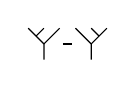
\begin{tikzpicture}[scale=.2]
	\path[draw] (0,0)--(0,1)--(-1,2);
	\draw (0,1)--(1,2);
	\draw (-.5,1.5)--(0,2);
	\draw (1.2,1)--(1.8,1);
	\path[draw] (3,0)--(3,1)--(2,2);
	\draw (3,1)--(4,2);
	\draw (3.5,1.5)--(3,2);	
	\end{tikzpicture}
\end{lrbox}
\newcommand{\associativity}{% <- this 'right of' is inherited; how to avoid?
	\usebox\preassociativity}

\newsavebox\precoassociativity
\begin{lrbox}{\precoassociativity}
	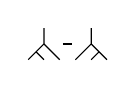
\begin{tikzpicture}[scale=.2]
	\path[draw] (0,0)--(0,-1)--(-1,-2);
	\draw (0,-1)--(1,-2);
	\draw (-.5,-1.5)--(0,-2);
	\draw (1.2,-1)--(1.8,-1);
	\path[draw] (3,0)--(3,-1)--(2,-2);
	\draw (3,-1)--(4,-2);
	\draw (3.5,-1.5)--(3,-2);
	\end{tikzpicture}
\end{lrbox}
\newcommand{\coassociativity}{% <- this 'right of' is inherited; how to avoid?
	\usebox\precoassociativity}

\newsavebox\preinvolution
\begin{lrbox}{\preinvolution}
	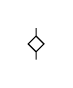
\begin{tikzpicture}[scale=.2]
	\path[draw] (0,0)--(0,.5)--(-.5,1)--(0,1.5)--(0,2);
	\path[draw] (0,.5)--(.5,1)--(0,1.5);
	\end{tikzpicture}
\end{lrbox}
\newcommand{\involution}{% <- this 'right of' is inherited; how to avoid?
	\usebox\preinvolution}

\newsavebox\preleftcounitality
\begin{lrbox}{\preleftcounitality}
	\begin{tikzpicture}[scale=.3]
	\draw (0,0)--(0,.8);
	\draw (0,0)--(.5,-.5);
	\draw (0,0)--(-.5,-.5);
	\draw [fill] (-.5,-.5) circle [radius=0.1];
	\draw (.7,0)--(1.1,0);
	\path[draw] (1.5,-.5)--(1.5,.8);
	\end{tikzpicture}
\end{lrbox}
\newcommand{\leftcounitality}{% <- this 'right of' is inherited; how to avoid?
	\usebox\preleftcounitality}

\newsavebox\preleftcounitcoproduct
\begin{lrbox}{\preleftcounitcoproduct}
	\begin{tikzpicture}[scale=.3]
	\draw (0,0)--(0,.8);
	\draw (0,0)--(.5,-.5);
	\draw (0,0)--(-.5,-.5);
	\draw [fill] (-.5,-.5) circle [radius=0.1];
	\end{tikzpicture}
\end{lrbox}
\newcommand{\leftcounitcoproduct}{% <- this 'right of' is inherited; how to avoid?
	\usebox\preleftcounitcoproduct}

\newsavebox\prerightcounitality
\begin{lrbox}{\prerightcounitality}
	\begin{tikzpicture}[scale=.3]
	\draw (0,0)--(0,.8);
	\draw (0,0)--(.5,-.5);
	\draw (0,0)--(-.5,-.5);
	\draw [fill] (.5,-.5) circle [radius=0.1];
	\draw (-.7,0)--(-1.1,0);
	\path[draw] (-1.5,-.5)--(-1.5,.8);
	\end{tikzpicture}
\end{lrbox}
\newcommand{\rightcounitality}{% <- this 'right of' is inherited; how to avoid?
	\usebox\prerightcounitality}

\newsavebox\prerightcounitcoproduct
\begin{lrbox}{\prerightcounitcoproduct}
	\begin{tikzpicture}[scale=.3]
	\draw (0,0)--(0,.8);
	\draw (0,0)--(.5,-.5);
	\draw (0,0)--(-.5,-.5);
	\draw [fill] (.5,-.5) circle [radius=0.1];
	\end{tikzpicture}
\end{lrbox}
\newcommand{\rightcounitcoproduct}{% <- this 'right of' is inherited; how to avoid?
	\usebox\prerightcounitcoproduct}

\newsavebox\preleftunitality
\begin{lrbox}{\preleftunitality}
	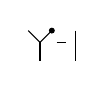
\begin{tikzpicture}[scale=.3]
	\draw (0,0)--(0,-.8);
	\draw (0,0)--(-.5,.5);
	\draw (0,0)--(.5,.5);
	\draw [fill] (.5,.5) circle [radius=0.1];
	\draw (.7,0)--(1.1,0);
	\path[draw] (1.5,.5)--(1.5,-.8);
	\end{tikzpicture}
\end{lrbox}
\newcommand{\leftunitality}{% <- this 'right of' is inherited; how to avoid?
	\usebox\preleftunitality}

\newsavebox\prerightunitality
\begin{lrbox}{\prerightunitality}
	\begin{tikzpicture}[scale=.3]
	\draw (0,0)--(0,-.8);
	\draw (0,0)--(-.5,.5);
	\draw (0,0)--(.5,.5);
	\draw [fill] (-.5,.5) circle [radius=0.1];
	\draw (-.7,0)--(-1.1,0);
	\path[draw] (-1.5,.5)--(-1.5,-.8);
	\end{tikzpicture}
\end{lrbox}
\newcommand{\rightunitality}{% <- this 'right of' is inherited; how to avoid?
	\usebox\prerightunitality}

\newsavebox\preproductcounit
\begin{lrbox}{\preproductcounit}
	\begin{tikzpicture}[scale=.3]
	\draw (0,0)--(0,-.8);
	\draw (0,0)--(.5,.5);
	\draw (0,0)--(-.5,.5);
	\draw [fill] (0,-.8) circle [radius=0.1];
	\end{tikzpicture}
\end{lrbox}
\newcommand{\productcounit}{% <- this 'right of' is inherited; how to avoid?
	\usebox\preproductcounit}

\newsavebox\preunitcoproduct
\begin{lrbox}{\preunitcoproduct}
	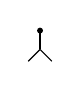
\begin{tikzpicture}[scale=.3]
	\draw (0,0)--(0,.8);
	\draw (0,0)--(.5,-.5);
	\draw (0,0)--(-.5,-.5);
	\draw [fill] (0,.8) circle [radius=0.1];
	\end{tikzpicture}
\end{lrbox}
\newcommand{\unitcoproduct}{% <- this 'right of' is inherited; how to avoid?
	\usebox\preunitcoproduct}

\newsavebox\preleibniz
\begin{lrbox}{\preleibniz}
	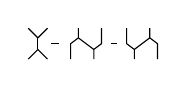
\begin{tikzpicture}[scale=.245]
	\draw (0,.3)--(0,-.3);
	\draw (0,.3)--(.5,.8);
	\draw (0,.3)--(-.5,.8);
	\draw (0,-.3)--(0,.3);
	\draw (0,-.3)--(.5,-.8);
	\draw (0,-.3)--(-.5,-.8);
	
	\draw (.7,0)--(1.1,0);
	\draw (2.1,.8)--(2.1,.3)--(1.7,0)--(1.7,-.8);
	\draw (2.1,.3)--(2.9,-.3);
	\draw (3.3,.8)--(3.3,0)--(2.9,-.3)--(2.9,-.8);
	
	\draw (3.8,0)--(4.1,0);
	\draw (4.6,.8)--(4.6,0)--(5,-.3)--(5,-.8);
	\draw (5,-.3)--(5.8,.3);
	\draw (5.8,.8)--(5.8,.3)--(6.2,0)--(6.2,-.8);	
	\end{tikzpicture}
\end{lrbox}
\newcommand{\leibniz}{% <- this 'right of' is inherited; how to avoid?
	\usebox\preleibniz}

\newsavebox\prebialgebra
\begin{lrbox}{\prebialgebra}
	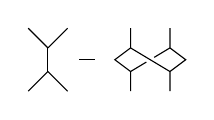
\begin{tikzpicture}[scale=.5]
	\draw (0,.3)--(0,-.3);
	\draw (0,.3)--(.5,.8);
	\draw (0,.3)--(-.5,.8);
	\draw (0,-.3)--(0,.3);
	\draw (0,-.3)--(.5,-.8);
	\draw (0,-.3)--(-.5,-.8);
	
	\draw (.8,0)--(1.2,0);
	
	\draw (2.1,.8)--(2.1,.3)--(1.7,0)--(2.1,-.3)--(2.1,-.8);
	
	\draw (3.1,.8)--(3.1,.3)--(3.5,0)--(3.1,-.3)--(3.1,-.8);

	\draw (2.1,.3)--(3.1,-.3);
	\draw (2.1,-.3)--(2.5,-.06);
	\draw (3.1,.3)--(2.7,.06);	
	\end{tikzpicture}
\end{lrbox}
\newcommand{\bialgebra}{% <- this 'right of' is inherited; how to avoid?
	\usebox\prebialgebra}

\newsavebox\precommutativity
\begin{lrbox}{\precommutativity}
	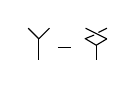
\begin{tikzpicture}[scale=.27]
	\draw (.3,0)--(.3,-1);
	\draw (.3,0)--(.8,.5);
	\draw (.3,0)--(-.2,.5);
	
	\draw (1.2,-.4)--(1.8,-.4);
	
	\draw (3,-.3)--(3,-1);
	\draw (2.5,0)--(3,-.3);
	\draw (3.5,0)--(3,-.3);
	\draw (2.46,0)--(2.9,.18);
	\draw (3.1,.3)--(3.5,.5);
	\draw (3.5,0)--(2.5,.5);
		\end{tikzpicture} 
	\end{lrbox}
	\newcommand{\commutativity}{% <- this 'right of' is inherited; how to avoid?
		\usebox\precommutativity}	

\begin{document}
\title{The cobar constructions as an $E_\infty$ Hopf algebra}
\author{Anibal M. Medina-Mardones}
\address{Max Plank Institute for Mathematics, Bonn, Germany}
\email{ammedmar@mpim-bonn.mpg.de}
\address{Department of Mathematics, University of Notre Dame, Notre Dame, IN, USA}
\email{amedinam@nd.edu}
\author{Your name}
\address{Your address}
\email{Your email}

\keywords{.}
\subjclass[2020]{.}

\begin{abstract}
	
\end{abstract} 

\vspace*{-1cm}

\maketitle

\tableofcontents

% !TEX root = ../cobar1.tex

\section{Introduction}

For any topological space $\fX$, its complex of simplicial or cubical singular chains $\Schains(\fX)$ -- regarded as a differential graded (dg) abelian group -- encodes the homology of $\fX$ in its quasi-isomorphism type.
More homotopical information can be stored in the quasi-isomorphism type of this chain complex if considered as a (coassociative) coalgebra, which we will denote $\SchainsA(\fX)$, where the coproduct comes from a natural choice of chain approximation to the diagonal $\fX \to \fX \times \fX$.
For instance, the cohomology ring of $\fX$ is retained, but the action of the Steenrod algebra on its mod~$p$ cohomology is not.

In Mandell's seminal work \cite{mandell2006homotopy_type} it is shown that, when $\fX$ is nilpotent and finite type, the entire homotopy type of $\fX$ can be encoded in the quasi-isomorphism type of this complex if considered as an $E_\infty$-coalgebra, a structure providing $\SchainsA(\fX)$ with coherent homotopies witnessing the derived cocommutativity of the coproduct coming from the strict symmetry of the diagonal map.

The first contribution of this paper is to explicitly endow the cubical singular chains of the based loop space $\loops_x \fX$, with the structure of a monoidal $E_\infty$-coalgebra extending the Serre diagonal.
More specifically, we verify that the monoid structure induced on $\cSchains(\loops_x \fX)$ by the concatenation of loops is compatible with a natural $E_\infty$-coalgebra structure on cubical singular chains, similar to the one defined in \cite{medina2022cube_einfty}.

Applying Adams' cobar construction to the coalgebra of simplicial singular chains of $(\fX, x)$, one obtains another monoidal algebraic model $\cobar \sSchainsA(\fX, x)$ of $\loops_x \fX$ \cite{adams1956cobar}.
More precisely, Adams constructed a natural monoidal chain map $\theta$ from $\cobar \sSchainsA(\fX, x)$ to $\cSchains(\loops_x \fX)$ and proved it to be a quasi-isomorphism if $\fX$ is simply-connected, a statement that also holds true for path-connected spaces after \cite{rivera2018cubical}.
The model $\cobar \sSchainsA(\fX, x)$ is smaller than $\cSchains(\loops_x \fX)$ and unlocks effective analysis of quantitative and qualitative properties of $\loops_x \fX$, as illustrated for instance in \cite{chainalgebraloops} and \cite{adamscobarequivalence}.

The second main contribution of this paper is to make Adams model into a monoidal $E_\infty$-coalgebra and to prove that
\[
\theta \colon \cobar \sSchainsA(\fX, x) \to \cSchains(\loops_x \fX)
\]
respects this higher structure.
Although not pursued in the present article, we remark that the explicit nature of our $E_\infty$-extension invites the study of primary and secondary operations for loops spaces using Adams' model and the tools developed in \cite{medina2021may_st}, \cite{medina2020cartan}, \cite{medina2021adem}, and \cite{medina2021comch}.

Our starting point is groundbreaking work by Baues, which imply statements similar to those in this work but in the category of (coassociative) coalgebras.
Baues reinterpreted Adams' algebraic construction at a deeper geometric level \cite{baues1998hopf}, which allowed him to endow $\cobar \sSchainsA(\fX, x)$ with the structure of a monoidal coalgebra, and to show that $\theta$ preserves this structure.
To prove our statement we interpret Adams' construction at an even deeper categorical level.
We interpret Baues' geometric cobar construction, originally defined for $1$-reduced simplicial sets, as a functor
\begin{equation*}
	\ccobar \colon \sSet^0 \to \Mon_{\cSet},
\end{equation*}
from the category of $0$-reduced simplicial sets to that of monoidal cubical sets.
The key difference with Baues' original work is the use of connections to obtain a natural construction before geometric realization.

Additionally, we need a suitable model of the $E_\infty$-operad endowing cubical chains with a natural $E_\infty$-coalgebra extending the Serre diagonal.
For this we take the operad $\UM$ introduced in \cite{medina2020prop1}.
After proving that its coalgebras form a monoidal category, we show that the functor $\cchainsUM \colon \cSet \to \coAlg_\UM$ -- defined in \cite{medina2022cube_einfty} with a different sign convention -- is monoidal.
This allows us to construct the following extension of Adams and Baues' structures.

\begin{theorem*}
	The following diagram commutes up to natural isomorphisms:
	\[
	\begin{tikzcd} [row sep=small]
		& \Mon_{\coAlg_\UM} \arrow[d] \\
		\Mon_{\cSet} \arrow[ru, "\cchainsUM", out=70, in=180, near start] \arrow[r, "\cchainsA"]
		& \Mon_{\coAlg} \arrow[d] \\
		\sSet^0 \arrow[r, "\cobar \schainsA"] \arrow[u, "\ccobar"]
		& \Mon_{\Ch},
	\end{tikzcd}
	\]
	where the unlabeled arrows are forgetful functors.
\end{theorem*}

In the diagram of the above theorem, the arrow from $\sSet^0$ to $\Mon_{\Ch}$ is Adams' cobar construction, the one from $\sSet^0$ to $\Mon_{\coAlg}$ is Baues' enhancement, and the one from $\sSet^0$ to $\Mon_{\coAlg_{\UM}}$ is our lift.
Additionally, we prove the following statement about Adams's map.

\begin{theorem*}
	For any pointed space $(\fX, x)$,
	\[
	\theta \colon \cobar \sSchainsA(\fX, x) \to \cSchains(\loops_x \fX)
	\]
	is a quasi-isomorphism of monoidal $\UM$-coalgebras.
\end{theorem*}

The fact that $\theta$ respects the monoid structure in $\Ch$ was proven by Adams, whereas the compatibility of the monoid structure with the Serre coalgebra structure was established by Baues.
Our contribution is the compatibility of the monoid structure with a full $E_\infty$-coalgebra extension of Serre's coalgebra.
We also remark that, whereas both Adams and Baues worked in the setting where the underlying space is simply connected, the above theorem does not require any connectivity or finiteness hypotheses.

\subsection*{Related work}

Kadeishvili \cite{kadeishvili1999coproducts, kadeishvili2003cupi} explicitly described monoidal cup-$i$ coproducts on $\cobar \schainsA(X)$ extending Baues coalgebra.
Kadeishvili, as Baues, used cubical methods to define these coproducts and to compare them, in the $1$-connected setting, to cup-$i$ coproducts extending the Serre coalgebra structure on the cubical singular chains of the based loop space.
Additionally, there are several papers \cite{smirnov1990iterated, smith1994cobar, smith2000operads, kadeishvili1998iterating} that predict the existence of, but do not construct, an $E_\infty$-structure on the cobar construction on the chains of simply connected simplicial sets.

On the dual side, Fresse \cite{fresse2003hopf} provided the bar construction of an algebra over the surjection operad with the structure of a comonoid in the category of algebras over the Barratt--Eccles operad.
Additionally, in \cite{fresse2010bar} he used a model category structure on reduced operads \cite{berger2003modelcategory, hinich1997homologicalalgebra} to iterate the bar construction on algebras over cofibrant $E_\infty$-operads.

The use of coalgebras instead of algebras allows us to relate the cobar construction to the based loop space directly --via the Adams map-- without imposing restrictions on the underlying homotopy type, as done by Fresse.
Furthermore, by grounding our approach on the cubical perspective at the heart of Adams' and Baues' seminal papers, we are able to preserve the natural monoidal structures when defining our $E_\infty$-enhancements.
\section{Simplices, cubes, and necklaces}

Discuss simplicial sets, cubical sets, and necklical sets. Define their normalized chain complexes and the coassociative coalgebra structures.

\subsection{Simplices}

\subsection{Cubes}\ \\

short definition of cubical sets

geometric and algebraic realizations

Serre diagonal

\subsection{Necklaces}
\section{Operads and props} \label{s:operads and props}

We consider the category $\Ch$ of chain complexes of abelian groups as our base category, remarking that all definitions in this section apply to general closed symmetric monoidal categories.

\subsection{$\S$-modules and $\S$-bimodules} \label{ss:symmetric (bi)modules}

Recall that a group $G$ can be thought of as a category with a single object and only invertible morphisms. From this viewpoint, a left $G$-module (resp. right $G$-module or $G$-bimodule) is the same as a functor from $G$ (resp. $G^\op$ or $G \times G^\op$) to $\Ch$.

Let $\S$ be the category whose objects are the natural numbers and whose set of morphisms between $m$ and $n$ is empty if $m \neq n$ and is otherwise the symmetric group $\S_n$.
A \textit{left $\S$-module} (resp. right $\S$-module or $\S$-bimodule) is a covariant functor from $\S$ (resp. $\S^\op$ or $\S \times \S^\op$) to $\Ch$.
In this paper we prioritize left module structures over their right counterparts. As usual, taking inverses makes both perspectives equivalent.

The homomorphisms $\S_n \to \S_n \times \S_1$ and $\S_n^\op \to \S_1 \times \S_n^\op$ induce natural forgetful functors $\Uleft$ and $\Uright$ from the category of $\S$-bimodules to those of left and right $\S$-modules.

Given a chain complex $C$ define:
\begin{align*}
\End^C(r) &= \Hom(C, C^{\otimes r})
& \End_C(r) &= \Hom(C^{\otimes r}, C)
&\End^C_C(r, s) &= \Hom(C^{\otimes r}, C^{\otimes s})
\end{align*}
with their natural structures of left $\S$-module, right $\S$-module, and $\S$-bimodule respectively.
The natural forgetful functors from $\S$-bimodules to left and right $\S$-modules send $\End^C_C$ to $\End^C$ and $\End_C$ respectively.

\subsection{Composition structures} \label{ss:composition structure}

Operads an props are $\S$-modules and \mbox{$\S$-bimodules} respectively enriched with certain composition structures. These are best understood by abstracting the composition structure naturally present in the $\S$-module $\End^C$, naturally an operad, and the $\S$-bimodule $\End^C_C$, naturally a prop.

Succinctly, an operad $\mathcal O$ is an $\S$-module together with a collection of $R$-linear maps
\begin{equation*}
\mathcal O(r) \otimes \mathcal O(s) \to \mathcal O(r+s-1)
\end{equation*}
satisfying suitable associativity, equivariance and unitality conditions.
A prop $\mathcal P$ is an $\S$-bimodule together with two types of compositions; horizontal
\begin{equation*}
\mathcal P(r_1, s_1) \otimes \mathcal P(r_2, s_2) \to \mathcal P(r_1 + r_2, s_1 + s_2)
\end{equation*}
and vertical
\begin{equation*}
\mathcal P(r,s) \otimes \mathcal P(s, t) \to \mathcal P(r, t)
\end{equation*}
satisfying their own versions of associativity, equivariance and unitality.
For a complete presentation of these concepts we refer to Definition 11 and 54 of \cite{Markl08}.

We remark that the compositional structure of a prop $\mathcal P$ restricts to operad structures on $\Uleft(\mathcal P)$ and $\Uright(\mathcal P)$.

\subsection{Representations} \label{ss:representations}

A morphisms of operads or of props is simply a morphisms of their underlying $\S$-modules or $\S$-bimodules preserving the respective compositional structures.

Consider a chain complex $C$, an operad $\mathcal O$ and a prop $\mathcal P$. An $\mathcal O$-\textit{coalgebra} (resp. $\mathcal O$-\textit{algebra}) structure on $C$ is an operad morphism $\mathcal O \to \End^C$ (resp. $\mathcal O \to \End_C$), and a $\mathcal P$-\textit{bialgebra} structure on $C$ is a prop morphism $\mathcal P \to \End_C^C$.

We remark that the linear duality functor naturally transforms an $\mathcal O$-coalgebra structure on a chain complex into an $\mathcal O$-algebra structure on its dual.

\subsection{Free operads and props} \label{ss:free props}

As described for example in \cite{Markl08}, the \textbf{free prop} $F(M)$ generated by a \mbox{$\S$-bimodule} $M$ is constructed using open directed graphs with no directed loops that are enriched with a labeling described next. We think of each directed edge as built from two compatibly directed half-edges. For each vertex $v$ of a directed graph $G$, we have the sets $in(v)$ and $out(v)$ of half-edges that are respectively incoming to and outgoing from $v$. Half-edges that do not belong to $in(v)$ or $out(v)$ for any $v$ are divided into the disjoint sets $in(G)$ and $out(G)$ of incoming and outgoing external half-edges. For any positive integer $n$, let $\overline{n} = \{1,\dots,n\}$ and $\overline{0} = \emptyset$. For any finite set $S$, denote the cardinality of $S$ by $|S|$. The labeling is given by bijections  
\begin{equation*}
\overline{|in(G)|}\to in(G), \qquad
\overline{|out(G)|}\to out(G),
\end{equation*}
and
\begin{equation*}
\overline{|in(v)|}\to in(v), \qquad
\overline{|out(v)|}\to out(v),
\end{equation*}
for every vertex $v$.
We refer to the isomorphism classes of such labeled directed graphs with no directed loops as $(n,m)$\textbf{-graphs} denoting the set of these by $\G(m,n)$.
We use graphs immersed in the plane to represent elements in $\G(m,n)$, please see Figure \ref{f:immersion}.
We consider the right action of $\S_n$ and the left action of $\S_m$ on a $(n,m)$-graph given respectively by permuting the labels of $in(G)$ and $out(G)$. This action defines the $\S$-bimodule structure on the free prop
\begin{equation} \label{e:free prop}
F(M)(m,n) \ = \bigoplus_{\Gamma \in \G(m,n)} \bigotimes_{v \in Vert(\Gamma)} out(v) \otimes_{\S_q} M(p, q) \otimes_{\S_p} in(v),
\end{equation}
where we simplified the notation writing $p$ and $q$ for $\overline{|in(v)|}$ and $\overline{|out(v)|}$ respectively. The composition structure is defined by (relabeled) grafting and union.

\begin{tikzpicture}[scale=.6]
\draw (1,3.7) to (1,3); 

\draw (1,3) to [out=205, in=90] (0,0);

\draw [shorten >= 0cm] (.6,2.73) to [out=-100, in=90] (2,0);

\draw [shorten >= .15cm] (1,3) to [out=-25, in=30, distance=1.1cm] (1,1.5);
\draw [shorten <= .1cm] (1,1.5) to [out=210, in=20] (0,1);

\node at (1,3.9){};
\node at (0,-.32){};
\node at (2,-.32){};

\node at (3,1.5){$\sim$\ \ \ };
\end{tikzpicture}
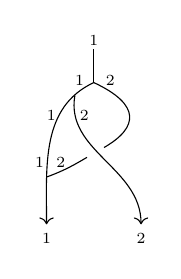
\begin{tikzpicture}[scale=.6]
\draw (1,3.7) to (1,3); 

\draw [->](1,3) to [out=205, in=90] (0,0);

\draw [shorten >= 0cm,->] (.6,2.73) to [out=-100, in=90] (2,0);

\draw [shorten >= .15cm] (1,3) to [out=-25, in=30, distance=1.1cm] (1,1.5);
\draw [shorten <= .1cm] (1,1.5) to [out=210, in=20] (0,1);


\def\x{.8}

\node[scale=\x] at (1,3.9){$\scriptstyle 1$};

\node[scale=\x] at (.7,3.05){$\scriptstyle 1$};
\node[scale=\x] at (1.35,3.05){$\scriptstyle 2$};

\node[scale=\x] at (.1,2.3){$\scriptstyle 1$};
\node[scale=\x] at (.8,2.3){$\scriptstyle 2$};

\node[scale=\x] at (-.15,1.3){$\scriptstyle 1$};
\node[scale=\x] at (.3,1.3){$\scriptstyle 2$};

\node[scale=\x] at (0,-.3){$\scriptstyle 1$};
\node[scale=\x] at (2,-.3){$\scriptstyle 2$};
\end{tikzpicture}

We remark that the free operad construction is described analogously using either graphs with a single input or output and only grafting.

\subsection{The prop $\M$} \label{ss:the prop M}

Let us consider the free prop $F(N)$ generated by the $\S$-bimodule $N$ whose only non-zero chain complexes are concentrated in degree $0$ and are give by
\begin{equation*}
N(1, 0)_0 = \Z\{\varepsilon\}, \qquad
N(1, 2)_0 = \Z[\S_2]\{\Delta\}.
\end{equation*}
Define $\A$ as the quotient of $F(N)$ by the prop ideal generated by the relations
\begin{equation*}
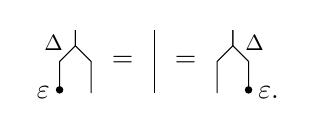
\begin{tikzpicture}[scale=.2]
\draw (-4,0)--(-4,2)--(-5,3)--(-5,4);
\draw (-6,0)--(-6,2)--(-5,3)--(-5,4);
\node [left, scale=.8] at (-5.3,3.2) {$\Delta$};
\draw [fill] (-6,.2) circle [radius=.2];
\node [left] at (-6,0) {$\varepsilon$};

\node at (-2,2) {=};
\draw (0,0)--(0,4);
\node at (2,2) {=};

\draw (4,0)--(4,2)--(5,3)--(5,4);
\draw (6,0)--(6,2)--(5,3)--(5,4);
\node [right, scale=.8] at (5.3,3.2) {$\Delta$};
\draw [fill] (6,.2) circle [radius=.2];
\node [right] at (6,0) {$\varepsilon$.};
\end{tikzpicture}
\end{equation*}
We remark that representations of the prop $\A$ correspond to counital coalgebra.

Let $W^{(1)}$ be the chain complex of free $\Z[\S_2]$-modules
\begin{equation*}
\begin{tikzcd}
\Z[\S_2]\{\nu\} &[0pt] \arrow[l, "1-T"'] \Z[\S_2]\{\mu\},
\end{tikzcd} 
\end{equation*}
which is isomorphic to the cellular chains on the standard model of the circle
\begin{equation*}
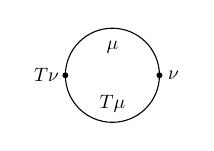
\begin{tikzpicture}[scale=.85]
\draw (0,0) circle (20pt);
\node[scale=.7] at (0,12pt){$\mu$};
\node[scale=.7] at (0,-12pt){$T \mu$};
\node[scale=.7] at (-28pt,0){$T \nu$};
\node[scale=.7] at (26pt,0){$\nu$};
\draw [fill] (-20pt,0) circle [radius=1pt];
\draw [fill] (20pt,0) circle [radius=1pt];
\end{tikzpicture}
\end{equation*}
and let $W^{(0)}$ be the subcomplex generated by $\nu$. We think of $W^{(1)}$ as an $\S_2$-equivariant 1-cell with boundary $W^{(0)}$.

We regard these complexes as $\S$-bimodules concentrated in biarity $(2,1)$, and let $\varphi \colon W^{(0)} \to \A$ be define by sending $T \nu$ and $\nu$ respectively to
\begin{equation*}
	\begin{tikzpicture}[scale=.2]
	\draw (-4,0)--(-4,4);
	\draw (-6,0)--(-6,4);
	\draw [fill] (-6,.2) circle [radius=.2];
	\node [left] at (-6,0) {$\varepsilon$};
	
	\node at (0,.4) {and};
	
	\draw (4,0)--(4,4);
	\draw (6,0)--(6,4);
	\draw [fill] (6,.2) circle [radius=.2];
	\node [right] at (6,0) {$\varepsilon$.};
	\end{tikzpicture}
\end{equation*}
Consider the push-out
\begin{equation*}
\begin{tikzcd}
F(W^{(0)}) \arrow[r, "F(\varphi)"] \arrow[d] & \A \arrow[d, dashed] \\
F(W^{(1)}) \arrow[r, dashed] & \mu \vee \A
\end{tikzcd}
\end{equation*}
in the category of props. We think of $\mathcal A \vee_\varphi \mu$ as the prop obtained by attaching a $1$-cell in biarity $(2,1)$ to $\A$.

Define $\M$ as the quotient of $\mu \vee \A$ by the ideal generated by
\begin{equation*}
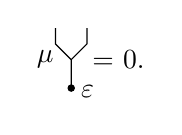
\begin{tikzpicture}[scale=.2]
\draw (5,4)--(5,3)--(6,2)--(6,0);
\draw (7,4)--(7,3)--(6,2);
\node [left] at (5.5,2) {$\mu$};
\draw [fill] (6,.2) circle [radius=.2];
\node [right] at (6,0) {$\varepsilon$};

\node at (9,2) {= 0.};
\end{tikzpicture}
\end{equation*}

We can give a more explicit description of $\M$ using the constructions of Subsection~\ref{ss:free props}.
Consider the $(m,n)$-graphs which we identify with $\varepsilon$, $\Delta$, and $\mu$:
\begin{equation*}
\counit \in \mathcal M(1,0)_0, \hspace*{.6cm} \coproduct \in \mathcal M(1,2)_0, \hspace*{.6cm} \product \in \mathcal M(2,1)_1.
\end{equation*}
Any element in $\M(m,n)$ can be written as a linear combination of the $(m,n)$-graphs generated by these three by grafting, disjoint union and relabeling.
The chain complex structure is determined using \eqref{e:free prop} by 
\begin{equation*}
\partial\ \counit = 0, \hspace*{.6cm} \partial \ \coproduct = 0, \hspace*{.6cm} \partial \ \product = \ \boundary \, ,
\end{equation*}
and is quotiented by the ideal generated by the relations
\begin{equation*}
\productcounit, \hspace*{.6cm} \leftcounitality \, , \hspace*{.6cm} \rightcounitality \, .
\end{equation*}

\subsection{The Hopf prop structure} \label{ss:hopf prop structure}

We now describe a diagonal map on $\M$, i.e., a chain map $\M(m,n) \to \M(m,n) \otimes \M(m,n)$ for every biarity $(m,n)$ compatible with the composition structure of $\M$.

As can be seen from \eqref{e:free prop}, the $(m,n)$-part of the free prop is defined only up to a choice of total order on the set of vertices of the $(m,n)$-graph involved.
Let $\Gamma \in \G(m,n)$ be a representative of an element in $\M(m,n)$ of degree $d$ and let us choose an order of its vertices.
This order defines a chain map
\begin{equation*}
\begin{tikzcd}[row sep=tiny]
\chains(\square^1)^{\otimes d} \arrow[r, "\iota_\Gamma"] & \M(m,n) \\
{[0,1]}^{\otimes d} \arrow[r, |->] & \Gamma.
\end{tikzcd}
\end{equation*}
We define the value of diagonal of $\M$ on $\Gamma$ using the Serre diagonal
\begin{equation} \label{e:diagonal of M}
\Delta(\Gamma) = \iota_\Gamma^{\otimes 2} \circ \Delta \left([0,1]^{\otimes d}\right).
\end{equation}
We need to show this is well defined.
It is independent of the choice of total order on $Vert(\Gamma)$ by Proposition~\ref{p:serre diagonal invariant}.
To prove the compatibility with the relations notice that ...
\section{The cobar construction}

Define the cobar construction of a connected dg coassociative coalgebra. 

Recall the construction of a coassociative associative bialgebra on the cobar construction of an $E_2$-coalgebra following Kadeishvhili/Matthias Franz. In fact, I think we can do this in the context of $U(M)$-coalgebras? Namely, if start with a $U(M)$-coalgebra then we may construct a coassociative coproduct on the cobar construction on the underlying $A_{\infty}$-coalgera by looking at its $E_2$ part.

Discuss the localized version of the cobar construction.
\section{A necklical model for the based loop space}

Construct a functor from simplicial sets to monoidal necklical sets modelling the based loop space functor. 

Discuss relationship with the cobar construction on the chains on a simplicial set. 

\section{Main theorem and applications}

Adams ...
\begin{equation*}
\begin{tikzcd}
& \Mon_{\Ch} \\
\sSet^1 \arrow[ru] \arrow[r, "\chains"] & \coAlg \arrow[u, "\cobar"]
\end{tikzcd}
\end{equation*}

Modeling the loop space. Category of $1$-reduced simplicial sets.

Baues lifted this construction through the forgetful functor $\coAlg \to \Ch$ to the category of coalgebras using a cubical monoid.

\begin{equation*}
\begin{tikzcd}
\Mon_{\cSet} \arrow[r, "\chains"] & \Mon_{\coAlg_R} \\
\sSet^0 \arrow[r, "\chains"] \arrow[u, "\gcobar"] & \coAlg_R \arrow[u, "\cobar"]
\end{tikzcd}
\end{equation*}

The algebraic structure on the simplicial chains responsible for the Baues diagonal on $\Omega \chains$ is referred to as a homotopy $G$-coalgebra, which corresponds to the $E_2$-structure on simplicial chains, naturally an $E_\infty$-coalgebra.
Later, Kadeishvili \cite{Kadeishvili03cup-i} extended this construction to produce cup-$i$ coproducts on the cobar construction. 
The simplicial chains carry the structure of a coalgebra over the surjection operad, and Fresse \cite{Fresse03construction} constructed on the cobar construction of a surjection coalgebra the structure of a Barratt-Eccles coalgebra.
Our result is most similar to Fresse's.
As it will become clear, two key differences are that he uses distinct operads for chains and their cobar construction and does not relate his construction to cubical cochains, a hallmark of Baues's insight.


%Applications: if the natural chain map between the normalized chains on a cubical set and its triangulation preserves the $U(M)$-coalgebra structure (check?) we may deduce that our model is equivalent as a $E_{\infty}$-bialgebra to the normalized chains on the classical Kan loop group functor (this would use recent work of Rivera, Zeinalian, and Minichello).


Us

\begin{equation*}
\begin{tikzcd}
\Mon_{\cSet} \arrow[r, "\chains"] & \Mon_{\coAlg_{U(\M)}} \\
\sSet^0 \arrow[r, "\chains"] \arrow[u, "\gcobar"] & \coAlg_{U(\M)} \arrow[u, "\cobar"]
\end{tikzcd}
\end{equation*} 

\bibliographystyle{alpha} % ieeetr
\bibliography{biblio}

\end{document}